% main.tex -- performance paper.  Every measured number in the text is a macro from numbers.tex,
% and every table/figure comes from make_perf.py, all generated from results/perf.json
% (bench_perf.py), results/arnoldi.json and results/convergence.json.
\documentclass[pre,twocolumn,superscriptaddress,longbibliography]{revtex4-2}
\usepackage{amsmath,amssymb,bm}
\usepackage{graphicx}
\usepackage{xcolor}
\usepackage[colorlinks=true,linkcolor=blue,citecolor=blue,urlcolor=blue]{hyperref}

\newif\ifaiauthor
\aiauthortrue           % \aiauthorfalse: arXiv/APS do not accept AI authors (see ../manuscript/PLAN.md, Sec. 6)
\newif\ifshowtodos
\showtodostrue
\newcommand{\todo}[1]{\ifshowtodos\textcolor{red}{[TODO: #1]}\fi}
\newcommand{\PT}{\mathcal{PT}}
\newcommand{\chit}{\chi^{(2)}}
\newcommand{\Img}{\mathrm{Im}\,}
\newcommand{\Rea}{\mathrm{Re}\,}
% generated by make_perf.py from results/perf.json, arnoldi.json -- do not edit
\newcommand{\modelErr}{+0}
\newcommand{\nCPU}{4}
\newcommand{\cpuName}{Intel Xeon Processor at 2.10GHz}
\newcommand{\numpyVer}{2.5.3}
\newcommand{\nStab}{4024}
\newcommand{\nNewton}{2016}
\newcommand{\pEig}{2.85}
\newcommand{\pInv}{2.84}
\newcommand{\pSolve}{2.46}
\newcommand{\tEigOne}{61}
\newcommand{\tEigFour}{29}
\newcommand{\tEigThree}{30}
\newcommand{\spEigFour}{2.11}
\newcommand{\spSolveFour}{2.10}
\newcommand{\pAmEig}{0.71}
\newcommand{\pAmSolve}{0.76}
\newcommand{\gfSolveOne}{60}
\newcommand{\gfSolveFour}{126}
\newcommand{\ratioEigSolve}{21}
\newcommand{\kCal}{1.09}
\newcommand{\pEigLocal}{2.96}
\newcommand{\peakCore}{67}
\newcommand{\gfInvOne}{43}
\newcommand{\gfInvFour}{95}
\newcommand{\spInvFour}{2.24}
\newcommand{\spEigThree}{2.00}
\newcommand{\spSolveThree}{2.25}
\newcommand{\thrVsSerial}{3.3}
\newcommand{\tEigTwoK}{8.3}
\newcommand{\ratioEigInv}{5.0}
\newcommand{\thrOneFour}{23.0}
\newcommand{\thrTwoTwo}{14.0}
\newcommand{\thrFourOne}{10.0}
\newcommand{\thrGain}{2.31}
\newcommand{\tEigRow}{65}
\newcommand{\tEigSpec}{33}
\newcommand{\shEigRow}{88}
\newcommand{\tRowTotal}{74}
\newcommand{\tAlpha}{4.9}
\newcommand{\nAlpha}{16}
\newcommand{\tBstep}{0.26}
\newcommand{\tJacAsm}{0.03}
\newcommand{\tJacSolve}{0.10}
\newcommand{\tPolish}{0.3}
\newcommand{\tArnTarget}{9.3}
\newcommand{\spArnTarget}{3.6}
\newcommand{\tConvMeas}{1741}
\newcommand{\tConvMeasMin}{29}
\newcommand{\tProjRun}{1748}
\newcommand{\tProjFourThr}{1669}
\newcommand{\tProjProc}{985}
\newcommand{\tProjArn}{655}
\newcommand{\spProjProc}{1.8}
\newcommand{\spProjArn}{2.7}
\newcommand{\usRKstep}{17}
\newcommand{\nRKsteps}{711}
\newcommand{\tRKshot}{0.01}
\newcommand{\usRHSscalar}{0.6}
\newcommand{\usRHSvecBig}{0.008}
\newcommand{\spRHS}{79}
\newcommand{\usSSFsmall}{353}
\newcommand{\gfSSFsmall}{1.63}
\newcommand{\gfSSFbig}{2.12}
\newcommand{\MSSFbig}{65536}
\newcommand{\spBatch}{2.4}
\newcommand{\KBatch}{16}
\newcommand{\KBatchMax}{64}
\newcommand{\spBatchMax}{1.6}
\newcommand{\usRHSvecOne}{8.6}
\newcommand{\gfSSFpeak}{2.8}
\newcommand{\MSSFpeak}{4096}
\newcommand{\gfSSFsmallest}{0.9}
\newcommand{\nShotsCaseOne}{1339}
\newcommand{\tFlowchart}{17}
\newcommand{\arAgree}{to the 6 significant digits stored}
\newcommand{\arN}{3016}
\newcommand{\arDense}{32.3}
\newcommand{\arTarget}{8.5}
\newcommand{\arScan}{248}
\newcommand{\tSpecProd}{27.6}
\newcommand{\modelRowErr}{23}
         % measured numbers (make_perf.py)

\begin{document}

\title{Where the time goes: performance anatomy of a pure-NumPy solver\\
for gap solitons in $\PT$-symmetric $\chit$ lattices}

\author{F. C. Moreira}
\affiliation{Universidade Federal de Alagoas, Macei\'o--AL, Brazil \todo{confirm affiliation}}
\ifaiauthor
\author{Claude Opus 5.5}
\affiliation{Anthropic (AI system); code, measurements and first draft produced in Claude Code}
\fi
\date{\today}

\begin{abstract}
We dissect the computational cost of the numerical chain of a companion study of gap solitons in a
quadratically nonlinear waveguide with a $\PT$-symmetric lattice. The chain consists of edge
shooting with adaptive Runge--Kutta--Fehlberg integration, Newton continuation on a symmetric half
domain, dense linear-stability spectra, and split-step Fourier propagation. It ran on a
\nCPU-core CPU without a GPU, with NumPy and OpenBLAS as the only numerical libraries. A
convergence study of five growth rates on three grids took \tConvMeasMin~minutes. Measurements
show that the dense nonsymmetric eigensolver takes \shEigRow\% of each row of that study. It scales
as $n^{\pEig}$ with the matrix size $n$. Four BLAS threads speed it up only $\times\spEigFour$, an
Amdahl parallel fraction of \pAmEig; on this virtual machine the LU kernels fare no better. The
production runs used no other form of parallelism. The other stages are cheap here but run far
from the arithmetic limit of the machine, bound by interpreter and memory overhead: a
Runge--Kutta step of the scalar shooting code costs \usRKstep~$\mu$s, and a split-step update on
$10^3$ points runs at \gfSSFsmall~GFLOP/s. We calibrate a task-scheduling model with the measured
kernels. It predicts that running the independent spectra as separate processes cuts the study
from \tProjRun~s to \tProjProc~s. Refining the large-box eigenvalues by shift-invert Arnoldi
iteration, instead of recomputing full spectra, brings it to \tProjArn~s. We list the changes in
order of gain per effort, with the measurements that justify each.
\end{abstract}

\maketitle

% =============================================================================================
\section{Introduction}
The companion paper \cite{Paper1} revisits the solitons of Ref.~\cite{MKM2013} with a numerical
chain written from scratch in Python \cite{NumPy2020}. The build environment had four cores of an
\cpuName, no GPU, no SciPy, no compiler toolchain for extensions, and no network access. The code
therefore implements every algorithm explicitly on top of NumPy \numpyVer\ and its bundled OpenBLAS.

Two production runs were slow enough to shape the study. Tracing five third-gap families with
spectra at every second point took 46 minutes. The convergence study that decides which growth
rates are physical took \tConvMeasMin~minutes: five points, three grids, two absorber strengths.
The question here is why. Which resources bound each stage? How much of the machine did the code
use? Which changes would pay off most? We answer with wall-clock measurements on the same machine
(Sec.~\ref{sec:method}), and turn them into a cost model that reproduces the production run and
projects alternatives (Sec.~\ref{sec:model}).

% =============================================================================================
\section{The pipeline and what bounds each stage}\label{sec:pipeline}
Figure~\ref{fig:pipeline} summarizes the chain, colour-coded by the resource that limits each
stage.

\emph{Edge shooting} integrates the stationary equations inward from the decaying Floquet tail,
with the Fehlberg 4(5) pair \cite{Fehlberg1969}. The state is four complex numbers, so each step is
a few dozen Python scalar operations. One shot takes \nRKsteps\ steps in \tRKshot~s, i.e.
\usRKstep~$\mu$s per step. The thesis flowchart needed \nShotsCaseOne\ shots for the semi-infinite
case 1, about \tFlowchart~s in total, so shooting is not where the time goes.

\emph{Newton continuation} solves for the $N=\nNewton$ real unknowns on the half grid. Each
iteration assembles a dense Jacobian (\tJacAsm~s) and solves it by LU decomposition (\tJacSolve~s).
Continuation is a chain: each step starts from the previous solution.

\emph{The stability spectrum} is the full spectrum of a dense complex non-Hermitian matrix of
size $n=4M=\nStab$ on the $L=40\pi$ box. It is computed by LAPACK's \texttt{zgeev}: reduction to
Hessenberg form, then the shifted QR algorithm \cite{LAPACK,GolubVanLoan}. Every point needs two
spectra, one per absorber strength.

\emph{Split-step propagation} applies two FFTs and a fourth-order Runge--Kutta local step per
update, to arrays of $M\approx10^3$ points; a run of $\zeta=1000$ has $10^5$ updates.

\begin{figure*}[t]
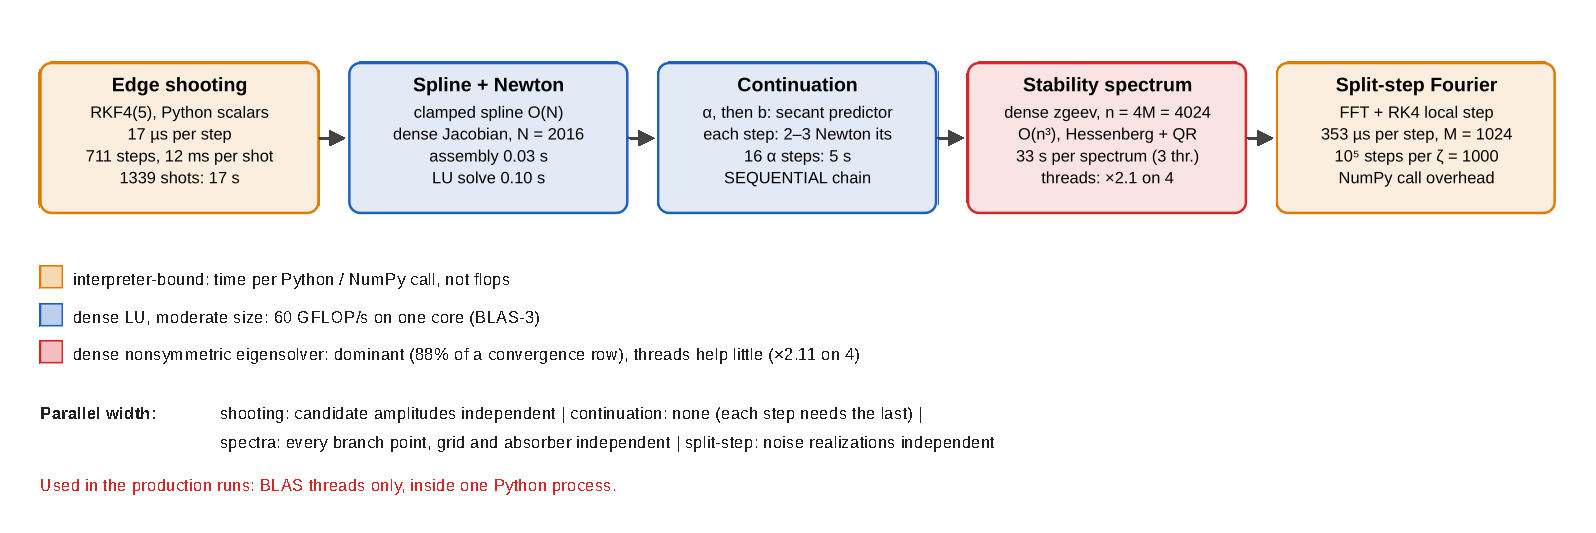
\includegraphics[width=\textwidth]{figures/fig_pipeline}
\caption{\label{fig:pipeline}The numerical chain with measured costs (L=$40\pi$, $h=0.25$). Orange:
the cost is the number of Python or NumPy calls, not floating-point work. Blue: dense linear algebra
of moderate size. Red: the dense nonsymmetric eigensolver, which dominates. The bottom lines list
the independent work available at each stage; the production runs used only BLAS threads.}
\end{figure*}

% =============================================================================================
\section{Measurement method}\label{sec:method}
All times are wall-clock times on an otherwise idle machine. Each kernel is the minimum over up to
three repetitions, the value least disturbed by other activity. OpenBLAS fixes its thread count
when NumPy is imported, so the benchmark driver starts a fresh child process for every thread
setting, with the environment variables set beforehand.

The dense kernels (Sec.~\ref{sec:dense}) are timed on random complex matrices, which isolates the
dependence on $n$. On the real stability matrix at $n=\nStab$, \texttt{zgeev} takes $\kCal$ times
as long as on a random matrix of the same size; the QR iteration count depends on the spectrum. The
cost model applies this calibration factor.

Flop counts follow the usual conventions for complex arithmetic \cite{GolubVanLoan}: $8n^3/3$ real
flops for an LU decomposition and $8n^3$ for an inverse. For the eigensolver we quote times only,
because its flop count depends on the number of QR sweeps. The script \texttt{bench\_perf.py}
reproduces every number; on this machine it takes under ten minutes.

% =============================================================================================
\section{Results}\label{sec:results}

\subsection{Dense kernels: cubic, and poorly threaded where it matters}\label{sec:dense}
Figure~\ref{fig:dense} and Table~\ref{tab:kernels} show the dense kernels. For $n\ge2000$ the
fitted exponents are \pEig\ (eigensolver), \pInv\ (inverse) and \pSolve\ (solve). Between the two
largest sizes the local exponent of the eigensolver is \pEigLocal, i.e.\ cubic, while the LU-based
kernels still gain efficiency as $n$ grows. At the production size $n=\nStab$, one spectrum costs
\tEigOne~s on one thread. That is \ratioEigSolve\ times the cost of an LU solve of the same matrix
and \ratioEigInv\ times the cost of an inverse.

Threads help every kernel about equally little. Four threads speed up the eigensolver by
$\times\spEigFour$, an Amdahl parallel fraction of \pAmEig~\cite{Amdahl1967}, and the LU solve by
$\times\spSolveFour$ (\pAmSolve). On one thread the LU solve runs at \gfSolveOne~GFLOP/s, close to
the AVX-512 peak of one core at 2.1~GHz, about \peakCore~GFLOP/s. On four threads it reaches
\gfSolveFour~GFLOP/s, roughly half of a four-core peak.

The guest system reports four cores without simultaneous multithreading. As a virtual machine,
however, its virtual CPUs may share physical cores or memory bandwidth on the host, and that cannot
be determined from inside. Whatever the cause, threads inside one kernel are worth about a factor of
two on this machine. For the eigensolver the cause is also algorithmic: a substantial part of its
Hessenberg reduction is matrix--vector work, and its QR sweeps apply chains of small rotations that
are inherently sequential \cite{GolubVanLoan}. Since it does \ratioEigSolve\ times the work of an
LU solve, it remains the bottleneck.

\begin{figure*}[t]
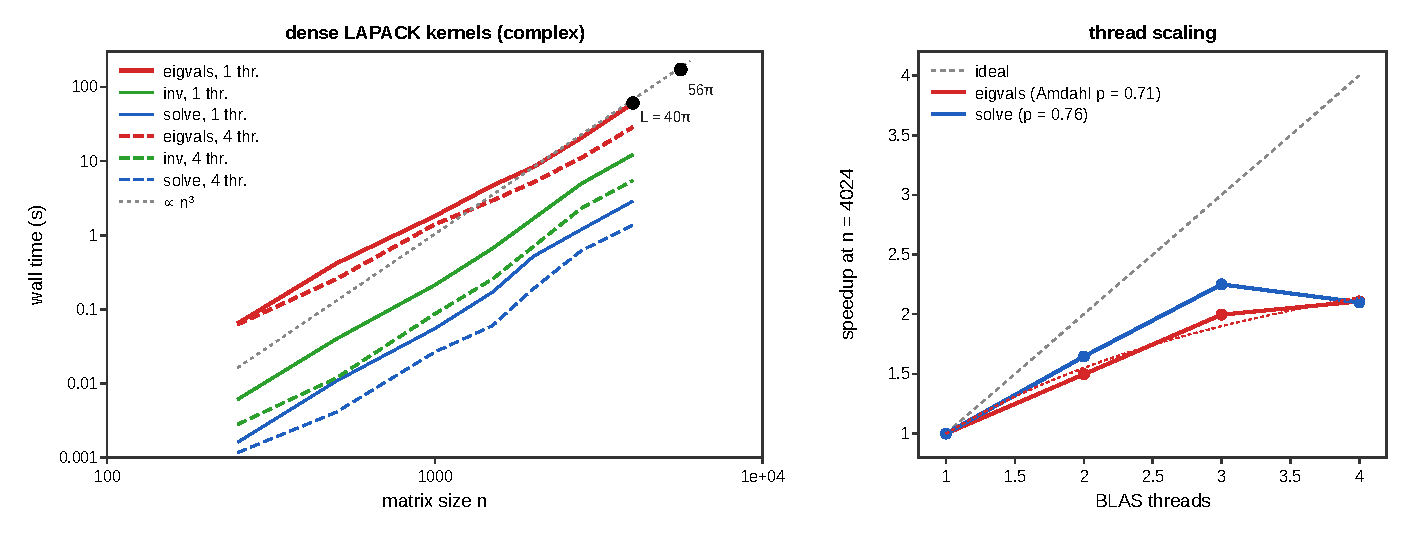
\includegraphics[width=0.9\textwidth]{figures/fig_dense}
\caption{\label{fig:dense}Left: wall time of the dense complex kernels against matrix size, for one
(solid) and four (dashed) BLAS threads; dotted: $\propto n^3$. Black dots: the stability-matrix
sizes of the production ($L=40\pi$) and large ($56\pi$) boxes. Right: speedup at $n=\nStab$ against
the number of threads, with Amdahl fits.}
\end{figure*}

\begin{table}[t]
\caption{\label{tab:kernels}Dense complex kernels: wall time (s) against $n$, and the LU flop rate
on one thread. The eigensolver timings are for random matrices.}
\footnotesize
% generated by make_perf.py -- do not edit
\begin{tabular}{rrrrrr}
\hline\hline
$n$ & eig, 1 thr. & eig, 4 thr. & inv, 1 thr. & solve, 1 thr. & solve GFLOP/s\\
\hline
1000 & 1.82 & 1.41 & 0.21 & 0.055 & 48.5\\
2000 & 8.32 & 5.19 & 1.68 & 0.519 & 41.1\\
2800 & 20.77 & 11.07 & 4.97 & 1.196 & 48.9\\
4024 & 60.84 & 28.87 & 12.25 & 2.894 & 60.0\\
\hline
fitted exponent & 2.85 & & 2.84 & 2.46 & \\
\hline\hline
\end{tabular}

\end{table}

\subsection{Anatomy of one convergence row}\label{sec:anatomy}
Table~\ref{tab:anatomy} and Fig.~\ref{fig:anatomy}(left) break down one row of the convergence
study: $\alpha=0.7919$, $b=-1.262$, on the $L=40\pi$ box with three threads, as in production. The
two spectra take \tEigRow~s, i.e.\ \shEigRow\% of the row. The edge shot, spline, Newton solves and
the \nAlpha-step $\alpha$ continuation together take the rest. Most of that rest is paid once per
grid, not once per row.

The right panel of Fig.~\ref{fig:anatomy} compares the measured wall time of each of the 15
production rows with the model of Sec.~\ref{sec:model}. The model counts, per row, the $b$
continuation, two calibrated spectra and, on the first row of each grid, the setup and the $\alpha$
chain. It reproduces the total to within \modelErr\%, and each row to within \modelRowErr\%.
The row scatter is run-to-run variation of the machine rather than of the model. Row 4 has exactly
the matrix of Table~\ref{tab:anatomy}, and its spectra took \tSpecProd~s each in the production run
against \tEigSpec~s in the benchmark. Wall times on this virtual machine therefore scatter by about
20\%, and the agreement of the totals is partly fortuitous. The large-box rows cost
about 2.4 times the production-box rows. That is less than $(56/40)^3\approx2.7$, because the
eigensolver is still below its asymptotic cubic scaling at three threads.

\begin{table}[t]
\caption{\label{tab:anatomy}Wall time per stage of one convergence row ($L=40\pi$, $h=0.25$,
Fourier, $n=\nStab$, 3 BLAS threads).}
\footnotesize
% generated by make_perf.py -- do not edit
\begin{tabular}{lrr}
\hline\hline
stage & time (s) & share\\
\hline
Floquet tails (monodromy, RKF45) & 0.04 & 0.1\%\\
shot: 2-D Newton polish & 0.33 & 0.4\%\\
shot: final profile & 0.08 & 0.1\%\\
Fourier $D_2$ and folding & 0.08 & 0.1\%\\
cubic spline & 0.01 & 0.0\%\\
Newton at $\alpha=0$ & 0.50 & 0.7\%\\
$\alpha$ continuation (16 steps) & 4.89 & 6.6\%\\
$b$ continuation (11 steps) & 2.82 & 3.8\%\\
spectrum, $g_0=1$ (zgeev) & 33.17 & 45.1\%\\
spectrum, $g_0=0.25$ (zgeev) & 31.65 & 43.0\%\\
\hline
total & 73.6 & 100\%\\
\hline
one Newton iteration: Jacobian assembly / dense solve & 0.03 / 0.10 & \\
Arnoldi, one shift (replaces one spectrum) & 9.33 & \\
\hline\hline
\end{tabular}

\end{table}

\begin{figure*}[t]
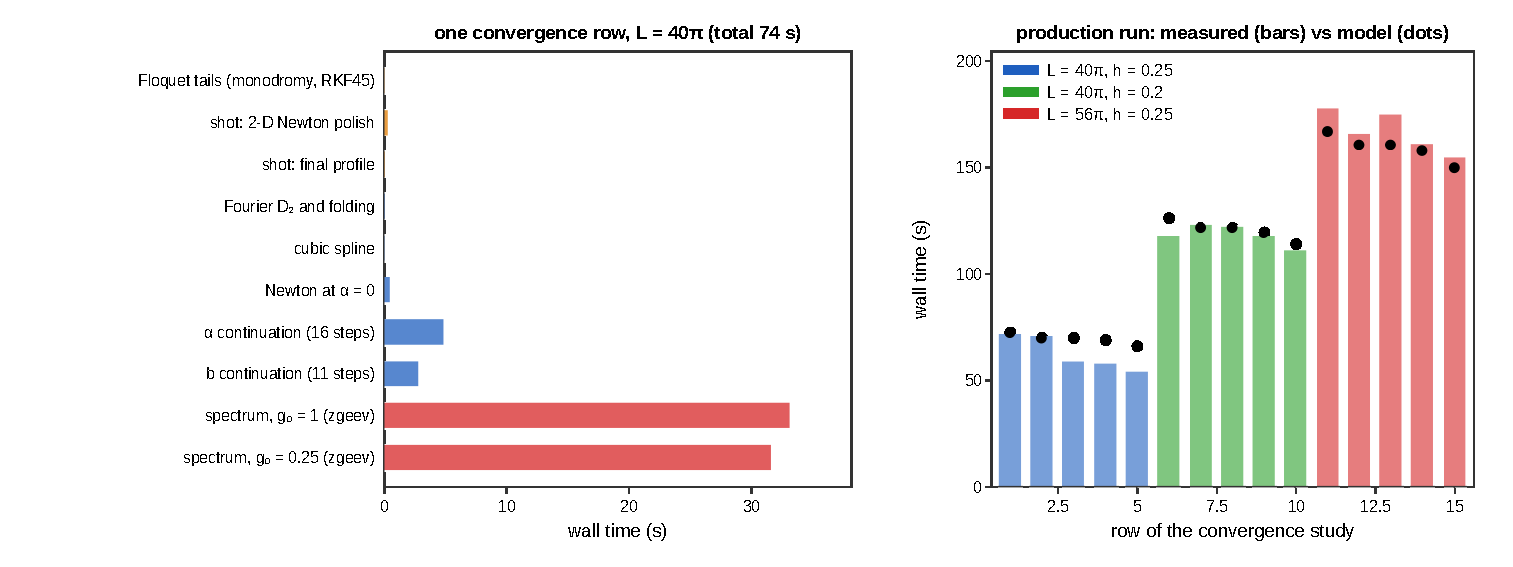
\includegraphics[width=\textwidth]{figures/fig_anatomy}
\caption{\label{fig:anatomy}Left: stages of one convergence row (red: spectra; orange: scalar
shooting; blue: Newton, continuation and setup). Right: measured wall time of the 15 rows of the
production run (bars, coloured by grid) against the calibrated cost model (dots).}
\end{figure*}

\subsection{Parallel structure, and what was used}\label{sec:parallel}
Figure~\ref{fig:dag} shows the task graph of the convergence study. The three grids are independent
lanes. Within a lane, the $\alpha$ chain is sequential, but after it the five $b$ chains are
independent. After its $b$ chain, each of the 30 spectra is independent.

The production run executed this graph as a single sequence of tasks in one process. Its only
parallelism was OpenBLAS threading inside each kernel, worth $\times\spEigFour$ at best on the
dominant one. Table~\ref{tab:throughput} measures the alternative directly on four independent
eigensolves of size 2000. One process with four threads takes \thrOneFour~s, and four single-thread
processes take \thrFourOne~s, $\times\thrGain$ more throughput. The four processes reach
\thrVsSerial\ times the throughput of a single one-thread process (\tEigTwoK~s per eigensolve),
close to linear. Separate processes sidestep the serial fraction of the eigensolver: each runs its
own sequential QR sweeps.

\begin{figure*}[t]
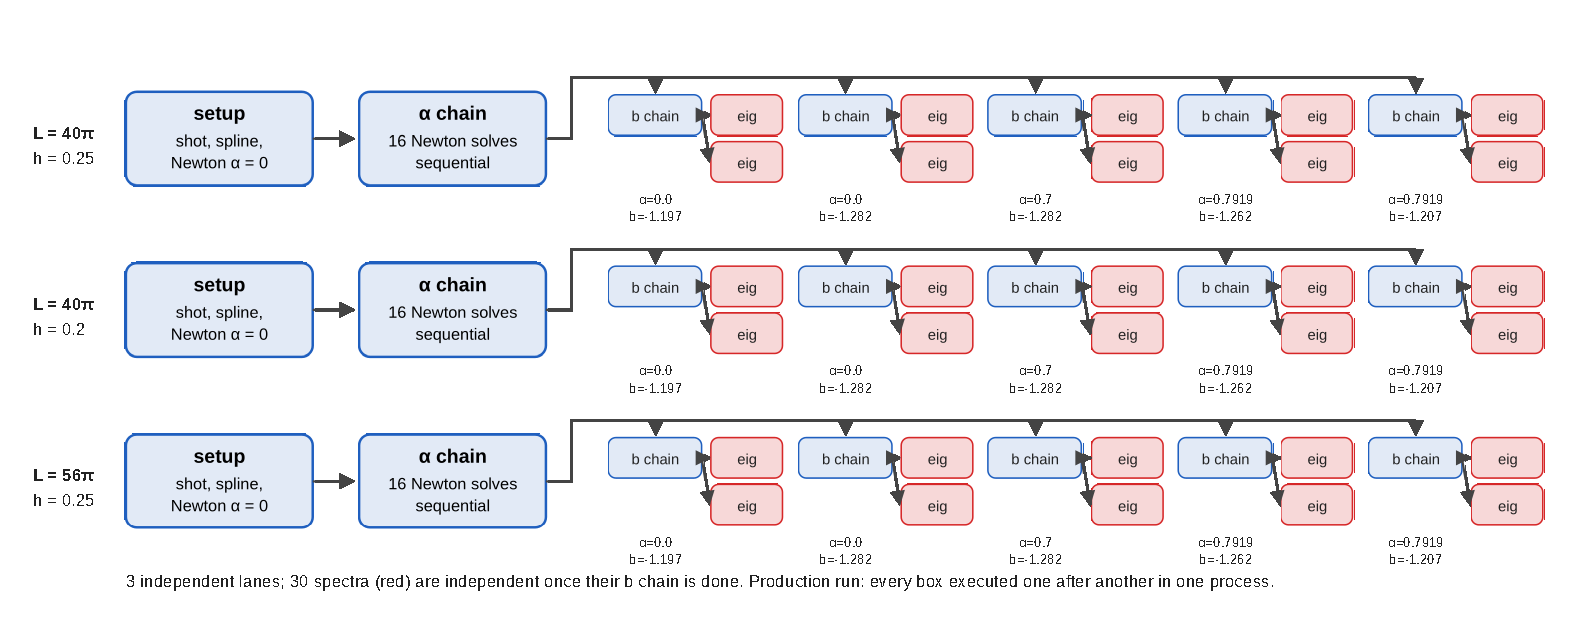
\includegraphics[width=\textwidth]{figures/fig_dag}
\caption{\label{fig:dag}Task graph of the convergence study. Each lane is one grid; after the
sequential $\alpha$ chain, the $b$ chains are independent, and every spectrum (red) depends only on
its own $b$ chain.}
\end{figure*}

\begin{table}[t]
\caption{\label{tab:throughput}Four independent eigensolves ($n=2000$): threads inside one process
against separate processes.}
\footnotesize
% generated by make_perf.py -- do not edit
\begin{tabular}{lrr}
\hline\hline
configuration (4 eigensolves, $n=2000$) & wall time (s) & relative\\
\hline
1 process $\times$ 4 threads, in series & 23.0 & 1.00\\
2 processes $\times$ 2 threads & 14.0 & 0.61\\
4 processes $\times$ 1 thread & 10.0 & 0.43\\
\hline\hline
\end{tabular}

\end{table}

\subsection{Interpreter-bound stages}\label{sec:interp}
In the scalar shooting code, one evaluation of the right-hand side costs \usRHSscalar~$\mu$s:
Python executes a few dozen complex operations, each through the interpreter. The same arithmetic
on NumPy arrays costs \usRHSvecOne~$\mu$s for a single state, because NumPy's fixed cost per call
dominates. Applied to 4096 states at once, it costs only \usRHSvecBig~$\mu$s per state, $\times\spRHS$
less than the scalar code; the break-even is near 16 states (Fig.~\ref{fig:interp}, right). The thesis flowchart marches $C_2$ over
many candidate values for each $C_1$. These shots are independent, so they can be integrated as one
array, with a common step size or with per-shot step control by masking.

The split-step update stays far from the arithmetic limit of the machine at every grid size
(Fig.~\ref{fig:interp}, left) \cite{Williams2009}. Its throughput rises from \gfSSFsmallest~GFLOP/s
at $M=256$ to \gfSSFpeak~GFLOP/s at $M=\MSSFpeak$, and falls again to \gfSSFbig~GFLOP/s at
$M=\MSSFbig$. For comparison, the LU solve runs at \gfSolveOne~GFLOP/s. At the production size
$M=1024$ a step costs \usSSFsmall~$\mu$s (\gfSSFsmall~GFLOP/s). At small $M$ the fixed cost of about
fifty NumPy calls per step dominates. At large $M$ the complex temporaries that every NumPy
operation allocates leave the cache, and memory traffic dominates.

Batching independent runs (noise realizations, parameter values) into one $(K,M)$ array gains at
most $\times\spBatch$, at $K=\KBatch$. At $K=\KBatchMax$ the gain drops to $\times\spBatchMax$ as the
arrays leave the cache. For this stage a compiled kernel that fuses the operations, or an FFT
library with batched plans \cite{FFTW2005}, would help more than batching in NumPy.

\begin{figure*}[t]
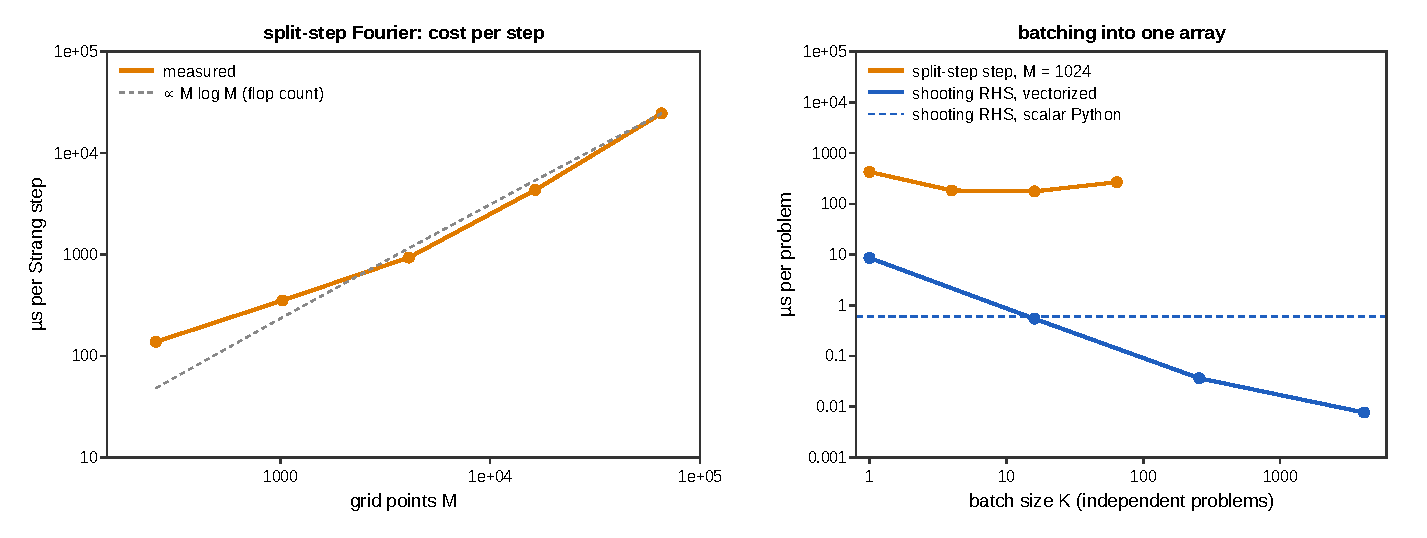
\includegraphics[width=0.9\textwidth]{figures/fig_interp}
\caption{\label{fig:interp}Left: split-step cost per Strang step against grid size; dotted: the
$M\log M$ flop count anchored at the largest size. Right: cost per problem when $K$ independent
problems share one array, for the split-step update ($M=1024$) and the shooting right-hand side,
against the scalar Python right-hand side (dashed).}
\end{figure*}

\subsection{Algorithmic alternatives to the dense spectrum}\label{sec:alg}
The growth rate needs only the few eigenvalues with the largest imaginary part, not all $n$ of them.
Shift-invert Arnoldi iteration \cite{Saad2011,ARPACK} with $(A-\sigma)^{-1}$ finds the eigenvalues
nearest a shift $\sigma$ in a few dozen steps. Our implementation restarts explicitly; a
Krylov--Schur restart \cite{Stewart2001} would converge in fewer steps. Without SciPy, the factorization is a dense inverse,
which on one core is \ratioEigInv\ times cheaper than the full spectrum.

Table~\ref{tab:arnoldi} compares three ways of getting the growth rate on the six test solitons of
the companion paper:
\begin{itemize}
\item the dense spectrum;
\item one shift next to a known eigenvalue, the use case of a larger-box refinement;
\item a blind scan with 26 shifts over $0\le\Rea\lambda\le3$.
\end{itemize}
All three agree, \arAgree. On the largest test
matrix ($n=\arN$), one shift takes \arTarget~s against \arDense~s for the dense spectrum. On the
$L=40\pi$ production matrix it is \tArnTarget~s against \tEigSpec~s, $\times\spArnTarget$ faster.
The blind scan needs one dense inverse per shift (\arScan~s), so without a sparse factorization it
is slower than the full spectrum.

The sparse factorization is where the real gain lies. With fourth-order finite differences, the
stability matrix has five nonzeros per row in each derivative block, plus diagonal couplings
(Fig.~\ref{fig:spy}). A sparse LU \cite{SuperLU}, through SciPy \cite{SciPy2020}, then costs
$O(n)$ rather than $O(n^3)$, and the blind scan becomes cheap. The code switches to this path
automatically when SciPy is present. It could not be run here, so its speedup is not measured.

The Fourier derivative, which the production runs used for its spectral accuracy, makes every
derivative block dense. The fourth-order differences reproduce the growth rate of the test soliton
to six digits (Table~\ref{tab:arnoldi}, first two rows). Choosing between the two derivatives is
therefore a choice between dense and sparse linear algebra.

\begin{table*}[t]
\caption{\label{tab:arnoldi}Growth rate and wall time of the dense spectrum, of shift-invert Arnoldi
at one shift next to the eigenvalue, and of the blind scan (26 shifts), NumPy backend, one thread,
for the six test solitons of the companion paper (results/arnoldi.json).}
\footnotesize
% generated by make_perf.py from results/arnoldi.json -- do not edit
\begin{tabular}{lrrrrr}
\hline\hline
soliton & $n$ & $\max\mathrm{Im}\,\lambda$ (dense) & dense (s) & one shift (s) & scan (s)\\
\hline
semi case 1, b=0.5 & 1504 & 0.179392 & 3.8 & 1.3 & 34\\
semi case 1, b=0.5, fd4 & 3016 & 0.179394 & 32.3 & 8.5 & 248\\
semi case 3, b=0.25 & 1504 & 0.109964 & 3.6 & 1.6 & 30\\
gap3 al=0, b=-1.197 & 2816 & 0.028108 & 19.5 & 6.4 & 196\\
gap3 al=0.7919, b=-1.207 & 2816 & 0.001035 & 20.9 & 7.0 & 202\\
gap3 al=0.7919, b=-1.101 & 2816 & 0.201048 & 22.0 & 7.7 & 212\\
\hline\hline
\end{tabular}

\end{table*}

\begin{figure*}[t]
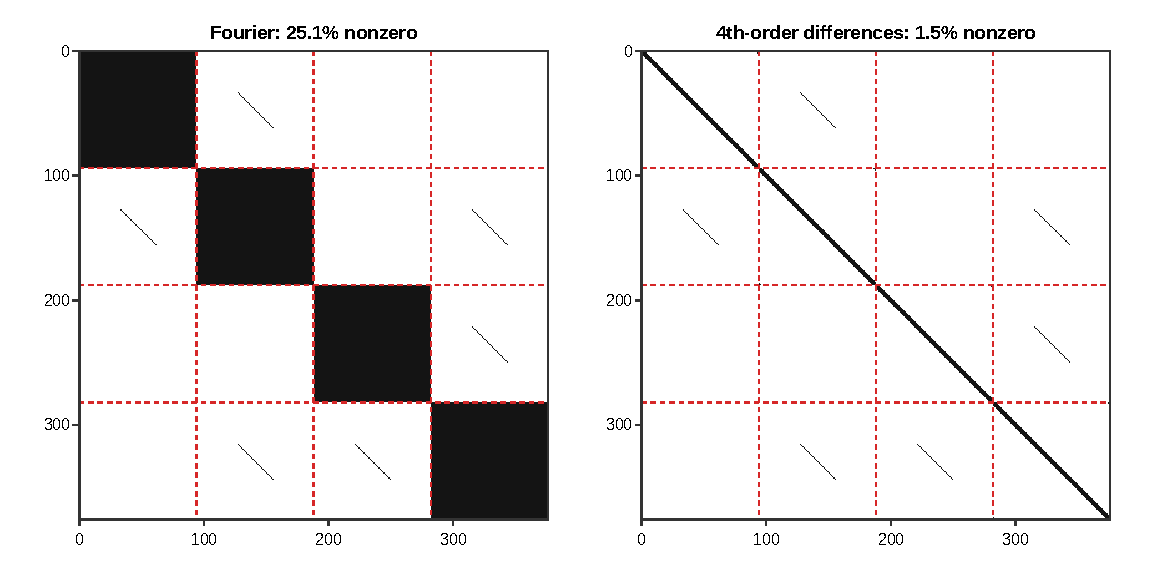
\includegraphics[width=0.75\textwidth]{figures/fig_spy}
\caption{\label{fig:spy}Nonzero pattern of the $4\times4$ block stability operator for a small box
(dashed: block boundaries). Left: Fourier differentiation, dense derivative blocks. Right:
fourth-order differences, banded blocks with periodic corners; a sparse LU factorization costs
$O(n)$.}
\end{figure*}

% =============================================================================================
\section{Cost model and projections}\label{sec:model}
Each task of Fig.~\ref{fig:dag} gets a duration from the measured kernels. A $b$-continuation step
costs \tBstep~s at $L=40\pi$, scaled by $N^3$ to other grids. A spectrum costs the calibrated
\texttt{zgeev} time at its $n$ and thread count. Setup and the $\alpha$ chain come from
Table~\ref{tab:anatomy}. The tasks are assigned to workers by greedy list scheduling: whenever a
worker is free, it takes the longest task whose dependencies are done \cite{Graham1969}.

For the production configuration (one worker, three threads) the model gives \tProjRun~s against
the measured \tConvMeas~s. Table~\ref{tab:projection} lists the projections:
\begin{itemize}
\item Using the fourth core through BLAS threads changes little.
\item Four single-thread processes: \tProjProc~s, $\times\spProjProc$. This is less than the
$\times\thrVsSerial$ throughput gain of Table~\ref{tab:throughput}. Single-thread spectra are
$\times\spEigThree$ slower than three-thread ones, and the sequential chains of each grid leave
workers idle at the start.
\item Adding the shift-invert refinement of the $L=56\pi$ eigenvalues, from guesses on the $40\pi$
box: \tProjArn~s, $\times\spProjArn$.
\end{itemize}

\begin{table}[t]
\caption{\label{tab:projection}Wall time of the 15-row convergence study predicted by the cost
model for four execution strategies, and the measured production run.}
\footnotesize
% generated by make_perf.py -- do not edit
\begin{tabular}{lrr}
\hline\hline
strategy & model wall time (s) & speedup\\
\hline
as run: 1 process, 3 BLAS threads, in series & 1748 & 1.0\\
1 process, 4 BLAS threads, in series & 1669 & 1.0\\
4 processes x 1 thread, task-parallel & 985 & 1.8\\
4 processes x 1 thread + Arnoldi refinement on the 56$\pi$ box & 655 & 2.7\\
\hline
measured production run (1 process, 3 threads) & 1741 & \\
\hline\hline
\end{tabular}

\end{table}

% =============================================================================================
\section{Recommendations}\label{sec:recommend}
In order of gain per effort:
\begin{enumerate}
\item \emph{Run independent spectra as separate single-thread processes.} This needs no change to
the numerics, only a process pool over the tasks of Fig.~\ref{fig:dag}. It is the largest gain of
the modelled strategies (Table~\ref{tab:projection}), and its building block is measured directly
(Table~\ref{tab:throughput}).
\item \emph{Refine known eigenvalues instead of recomputing spectra.} On larger boxes, finer grids,
and along a branch, the previous eigenvalue is a good shift; one shift-invert Arnoldi solve
replaces a full spectrum.
\item \emph{Use a sparse factorization.} With SciPy and the fourth-order derivative, each shift is
expected to cost $O(n)$; this is not measured here. That would remove the cubic bottleneck and make
much larger boxes affordable, as needed near band edges, where the solitons are wide.
\item \emph{Batch the shooting.} Integrate the candidate shots of the flowchart as one array; the
right-hand side gets $\times\spRHS$ cheaper per shot at 4096 shots (Sec.~\ref{sec:interp}). For
split-step propagation, NumPy batching gains only $\times\spBatch$.
\item \emph{Compile the inner loops}, e.g.\ with Numba \cite{Numba2015}: the scalar integrator
when batching is not possible, and the fused split-step update, which batching in NumPy does not
fix.
\item \emph{GPUs} are unlikely to help the dense nonsymmetric eigensolver at these sizes, because
its sequential parts dominate. They should help batched split-step propagation, which is FFT and
elementwise work \cite{FFTW2005}; we could not test this here.
\end{enumerate}

\section{Conclusions}
The convergence study was slow for three reasons. First, it computed full $O(n^3)$ spectra where a
few eigenvalues sufficed. Second, it left its task-level parallelism unused. Third, threads inside
one kernel give only about a factor of two on this machine. The first two are choices of the code,
not limits of the hardware. The third is a property of the virtual machine and of the eigensolver
(Amdahl fraction \pAmEig), and it is the reason separate processes pay more than threads. Each fix
is measured, or projected from measured kernels. Together they reduce the study from \tProjRun~s
to \tProjArn~s on the same four cores, before any sparse factorization.

\section*{Data and code availability}
\texttt{bench\_perf.py}, \texttt{make\_perf.py} and the measurement file \texttt{results/perf.json}
are in the repository of the companion paper \cite{Paper1}.

\begin{acknowledgments}
\todo{acknowledgments.}
\ifaiauthor\else
\emph{Use of AI.} The code, the measurements and a first draft were produced by the AI system Claude
Opus 5.5 (Anthropic) in Claude Code, under the direction of F.~C.~Moreira, who is responsible for
the content.
\fi
\end{acknowledgments}

\bibliography{refs}
\end{document}
